\chapter{Resultados}
\label{chap:resultados}

Este capítulo apresenta as análises e os resultados obtidos durante as etapas de validação empírica do sistema de telemetria desenvolvido. Para assegurar a rastreabilidade das falhas e a confiabilidade da arquitetura, a metodologia de ensaios foi segmentada de forma progressiva, partindo da verificação modular dos subsistemas lógicos e físicos até a homologação do arranjo completamente integrado.

A estrutura de avaliação divide-se em três frentes experimentais. Primeiramente, expõe-se a validação funcional dos componentes, detalhando o emprego de rotinas Hardware-in-the-Loop (HIL) e emuladores de rede para atestar a integridade do fluxo de dados isolado no nó embarcado, no middleware terrestre e, por conseguinte, na estação de solo (Odin). Em seguida, o texto aborda as características elétricas do sistema embarcado, analisando a estabilidade da regulação de tensão nos circuitos de alimentação, o perfil de consumo de corrente em regime de operação e o comportamento do hardware quando inserido na malha de potência compartilhada com o sistema de controle da aeronave.

Por fim, apresenta-se um ensaio de campo direcionado à camada física de radiofrequência, estruturado para mensurar a degradação da qualidade do enlace LoRa — expressa pelo indicador RSSI (Received Signal Strength Indicator) — em função da distância geométrica. O experimento submete o transceptor a condições de perda de linha de visada direta e interferências de relevo natural, simulando o perfil de atenuação esperado em um ambiente de voo real. O conjunto destas experimentações fundamenta a avaliação crítica sobre o cumprimento dos requisitos técnicos e as capacidades da solução proposta.


\section{Validação Funcional dos Componentes}
A validação do firmware embarcado na aeronave operou sob a metodologia Hardware-in-the-Loop (HIL), permitindo a verificação da lógica de domínio em isolamento das variabilidades físicas dos sensores. No primeiro cenário experimental, as tarefas ProducerUartHilTask e ConsumerUartHilTask substituíram as portas de hardware originais do sistema. O script data\_injector.py foi utilizado no computador host para sintetizar pacotes de telemetria, baseados em perfis de voo em formato CSV, e injetá-los no microcontrolador via barramento serial (USB UART). A camada de domínio processou as informações e as exportou através da porta de consumo emulada, onde foram capturadas e validadas no host. Esta etapa atestou a corretude das rotinas de quantização, a estabilidade da máquina de estados finita e a consistência do encapsulamento em estrutura MAVLink.

Em um segundo momento, a avaliação estendeu-se à validação da camada de comunicação em radiofrequência. A topologia foi reconfigurada mantendo o adaptador de produção simulado (ProducerUartHilTask) para a injeção contínua de dados, porém, a saída foi redirecionada para a tarefa física de transmissão via transceptor SX1276. Para aferir a integridade da transmissão, um segundo microcontrolador foi configurado como nó receptor, executando uma rotina de escuta (lora\_receptor.ino). O tráfego capturado no enlace LoRa foi encaminhado ao computador via interface serial e decodificado pelos scripts data\_consumer.py e serial\_monitor.py. A análise destes registros atestou a manutenção da integridade estrutural dos pacotes MAVLink após o processo de serialização via barramento SPI e posterior propagação eletromagnética.

A validação do componente middleware concentrou-se na análise de sua capacidade de atuar como ponte de roteamento ininterrupto entre o enlace LoRa e a rede local sem fio (Wi-Fi). Para certificar essa funcionalidade, o script listener.py foi executado para emular o comportamento de conexão passiva da estação de solo real. Acoplado à interface de rede, o simulador monitorou o tráfego de sockets consumindo os datagramas UDP roteados pelo middleware. A verificação de paridade entre a carga útil entregue ao script de escuta e os dados originais injetados pelo simulador HIL comprovou a ausência de perdas, fragmentações críticas ou bloqueios de tráfego (bottlenecks) na conversão de protocolos do subsistema de solo.

Por fim, a estação de controle em solo (Odin) e o ecossistema como um todo foram submetidos à homologação de integração. A arquitetura foi montada em sua configuração final de operação: o sistema embarcado operou sobre sensores reais (IMU, Barômetro e GPS), enviando a carga útil pelo transceptor LoRa ao middleware, que redirecionou o fluxo via roteamento Wi-Fi em pacotes UDP até a aplicação cliente. A estação de solo obteve êxito em estabelecer a escuta assíncrona, desserializar o fluxo binário em componentes lógicos, aplicar os filtros de reconstrução de escala nas variáveis cinemáticas e renderizar o painel gráfico de forma contínua, garantindo adicionalmente a persistência em disco rígido. O sucesso desta experimentação integrada consolidou a validação funcional, provando que as premissas arquiteturais de baixo acoplamento adotadas mitigaram efetivamente o acúmulo de latência entre a ponta aquisitiva e a ponta de monitoramento.


\section{Características Elétricas do Sistema Embarcado}

A garantia da integridade operacional do nó embarcado, bem como a prevenção de falhas catastróficas em voo, depende intrinsecamente da estabilidade de sua malha de alimentação e do correto dimensionamento do consumo energético. Para avaliar o comportamento elétrico do \textit{hardware} projetado, a primeira etapa de testes consistiu na aferição das tensões reguladas nos barramentos internos da placa, operando com uma bateria fornecendo tensão nominal de 6,55 V na entrada. A aferição via multímetro digital na trilha de saída do regulador linear (LDO) registrou um potencial de 3,29 V (Figura \ref{fig:medicao_tensoes}), o que certifica a alimentação adequada para a lógica de 3,3 V do microcontrolador ESP32 e dos barramentos de comunicação I2C/SPI. Simultaneamente, a trilha alimentada pelo módulo conversor \textit{buck} (Mini360) apresentou uma tensão aferida de 3,503 V. Este leve sobredimensionamento atende aos requisitos operacionais dos módulos periféricos sem violar os limites de tolerância absoluta dos componentes, validando a arquitetura de rebaixamento de tensão do projeto.

\begin{figure}[ht]
    \centering
    \caption{Aferição das Tensões no Sistema Embarcado}
    \label{fig:medicao_tensoes}
    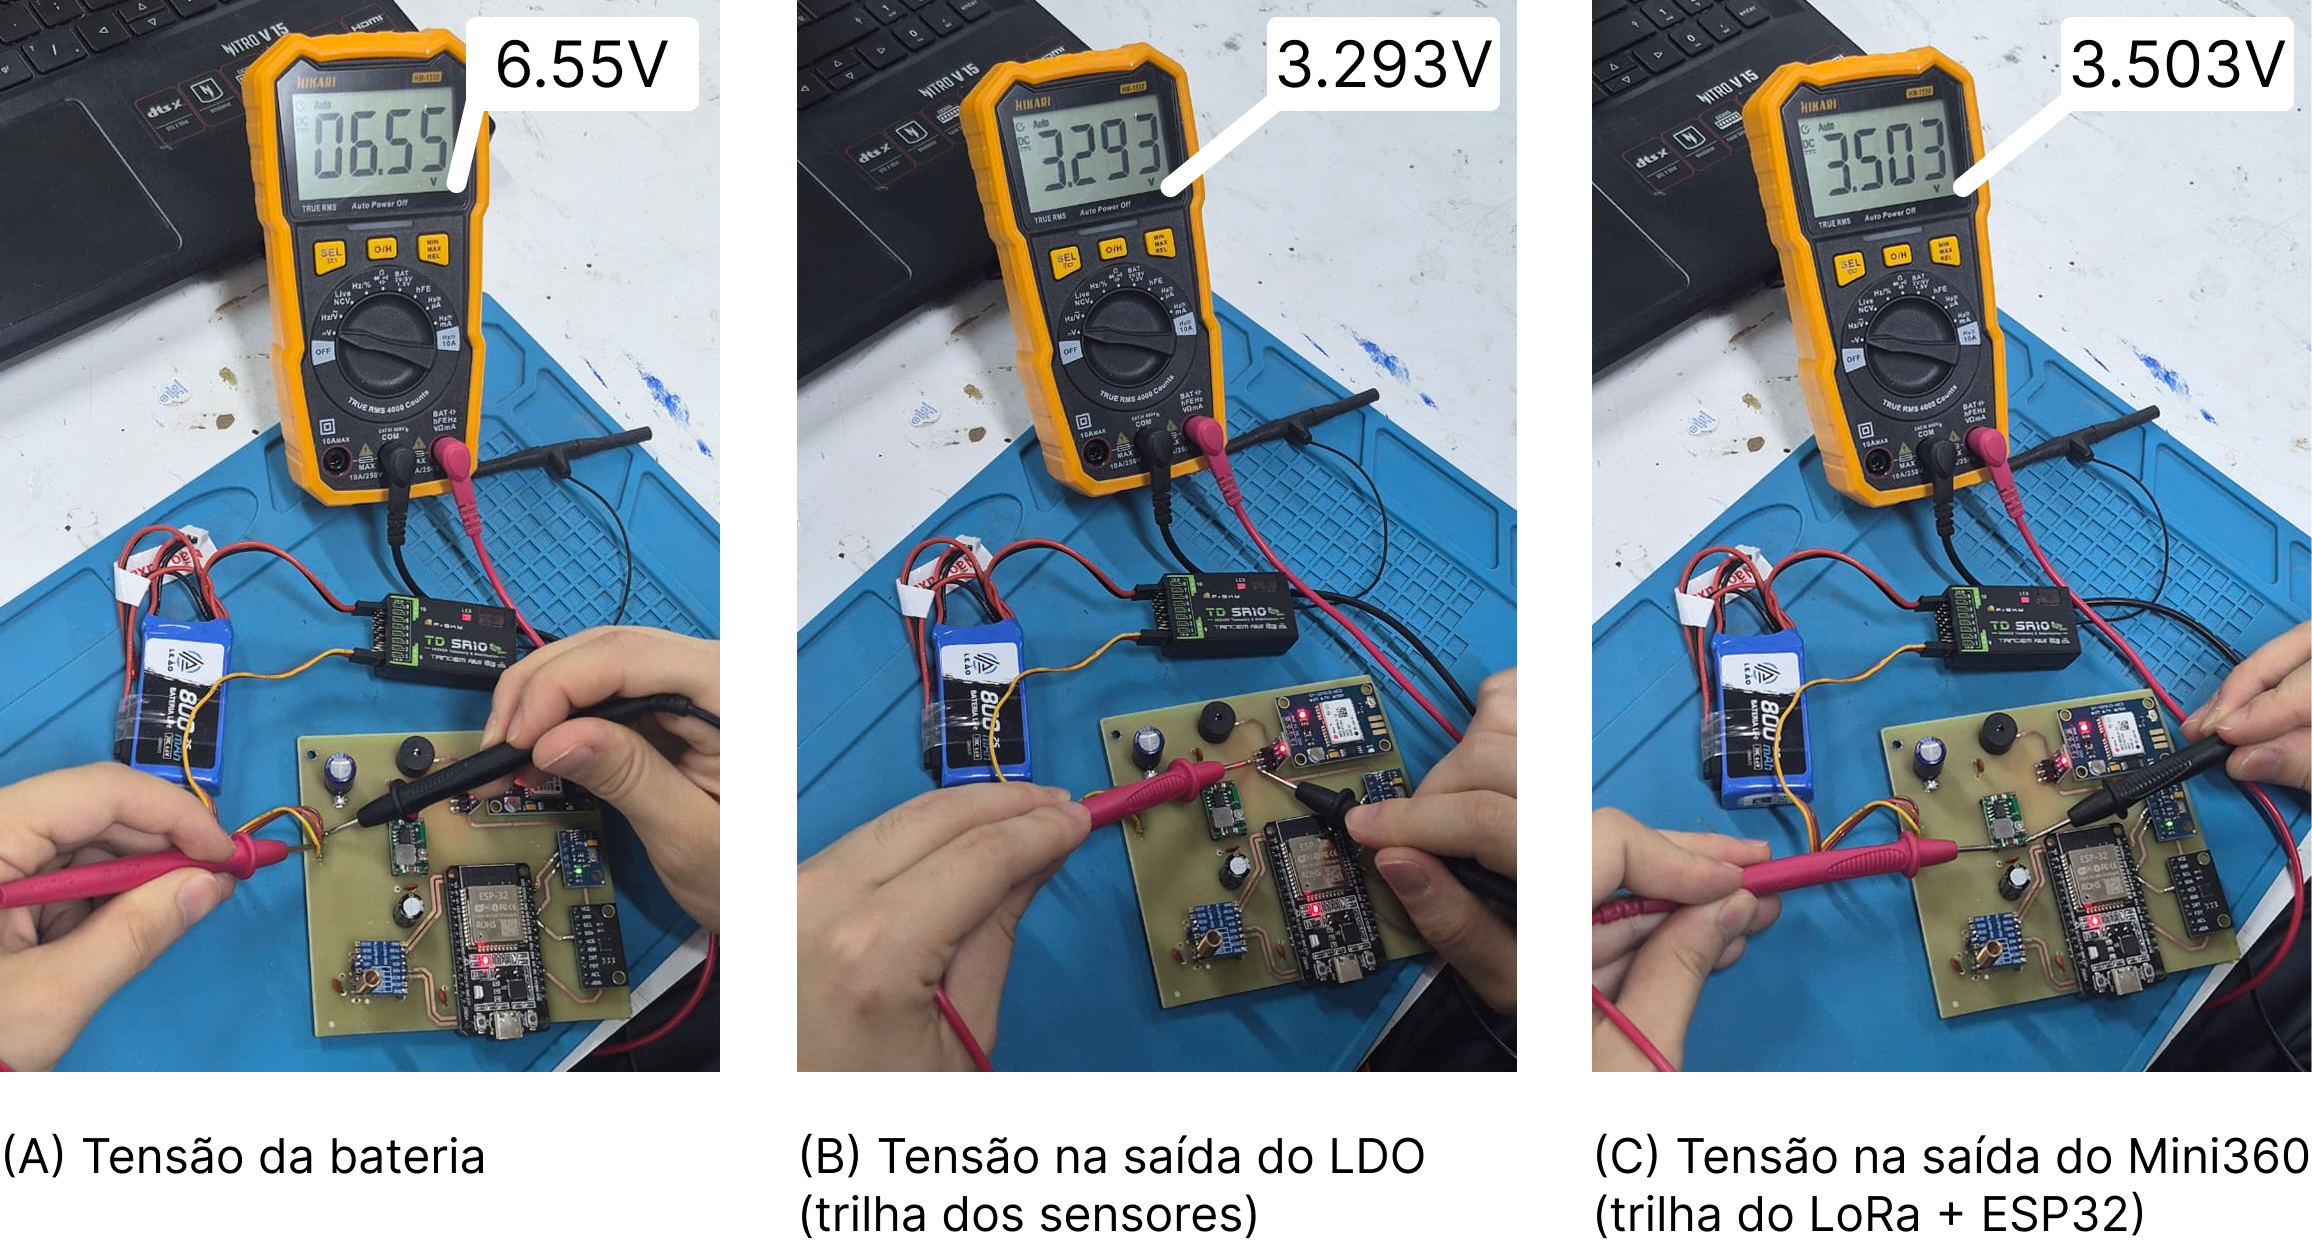
\includegraphics[width=1\textwidth]{images/tensao_pcb.png}\\
    \footnotesize Fonte: Autoria própria, 2026.
\end{figure}

No que tange ao perfil de consumo energético, o sistema foi monitorado em regime contínuo de captura sensorial e emissão de dados via radiofrequência. A instrumentação de medição indicou que o \textit{hardware} embarcado demanda uma corrente média de aproximadamente $0,033 A$ durante a maior parte do ciclo de execução. Contudo, a análise da curva de carga revelou a ocorrência de picos transitórios de corrente que atingem até $0,89 A$, conforme Figura \ref{fig:grafico_corrente}. Essa elevação abrupta e momentânea é uma característica esperada da modulação física do transceptor LoRa SX1276 (configurado para potência máxima de transmissão no estágio \textit{PA\_BOOST}), reafirmando a necessidade do barramento capacitivo e do conversor chaveado exclusivo para suprir as demandas instantâneas de rajada sem desestabilizar o barramento lógico primário.

\begin{figure}[ht]
    \centering
    \caption{Corrente do Sistema Embarcado ao Longo do Tempo}
    \label{fig:grafico_corrente}
    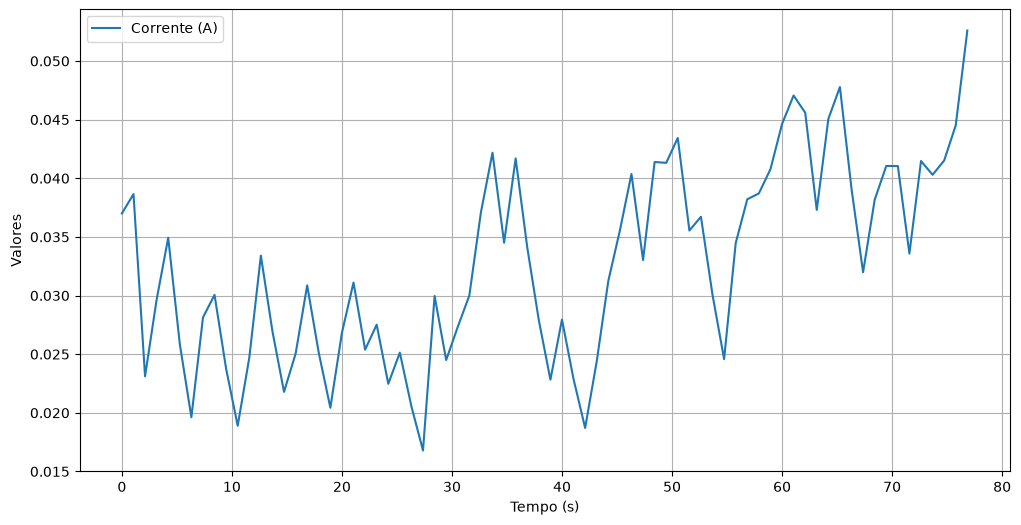
\includegraphics[width=1\textwidth]{images/corrente_embarcado.png}\\
    \footnotesize Fonte: Autoria própria, 2026.
\end{figure}

Por fim, a resiliência da arquitetura foi submetida a um ensaio de estresse com o sistema de telemetria integrado à malha de potência do sistema de controle da aeronave. O objetivo desta avaliação foi identificar potenciais afundamentos de tensão (\textit{sags}) ocasionados pelo acionamento concorrente dos servomotores e da comunicação. A análise do registro gráfico do teste indicou que, mesmo sob carga integrada, a tensão do barramento principal não decaiu consistentemente para valores inferiores a 5,0 V, conforme Figura \ref{fig:grafico_sistema_controle}.

\begin{figure}[ht]
    \centering
    \caption{Tensão e Corrente do Sistema de Controle}
    \label{fig:grafico_sistema_controle}
    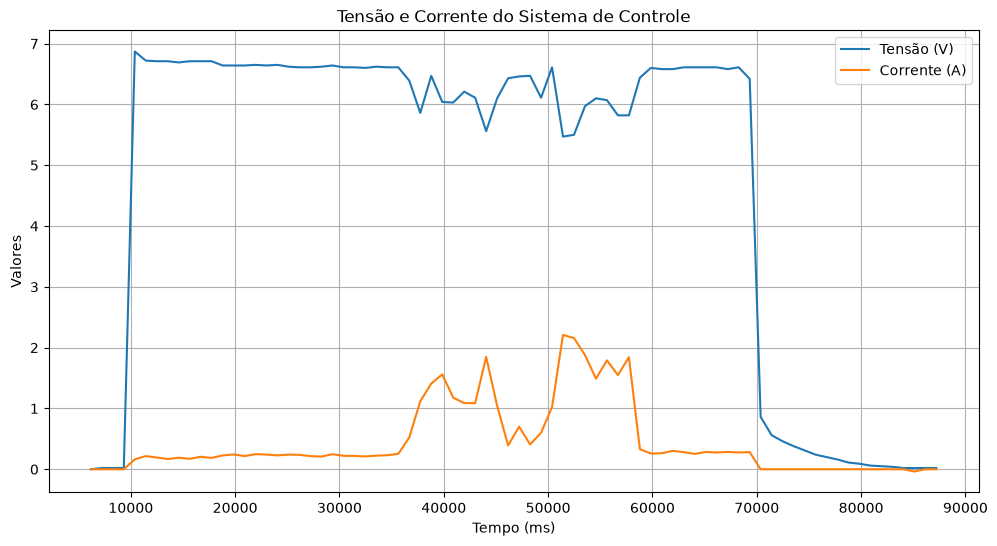
\includegraphics[width=1\textwidth]{images/grafico_sistema_controle.png}\\
    \footnotesize Fonte: Autoria própria, 2026.
\end{figure}

Ressalta-se, de forma crítica, que a taxa de amostragem inerente aos equipamentos de monitoramento utilizados para este ensaio específico pode mascarar quedas de tensão de alta frequência. Oscilações transientes na ordem de microssegundos podem não ter sido capturadas pelo histórico de medição. No entanto, a observação empírica corroborou a robustez do sistema elétrico: o microcontrolador operou sob constante monitoramento em modo \textit{debug} (via console) e não acusou, em momento algum, o acionamento do circuito supervisor de \textit{brownout detector} (BOD) ou reinicializações (\textit{resets}), comprovando que as flutuações de potência da aeronave não são suficientes para comprometer a estabilidade do \textit{firmware} de telemetria.


\section{Teste de Distância e Qualidade da Comunicação LoRa}

A confiabilidade do enlace de radiofrequência é um fator limitante para a operação segura de sistemas de telemetria aeroespacial. Para mensurar a resiliência da modulação LoRa adotada neste projeto, estruturou-se um ensaio de campo focado na avaliação da degradação do sinal — quantificada pelo Índice de Força do Sinal Recebido (RSSI) — em função do distanciamento geográfico entre a estação base e o nó transmissor.

O experimento foi conduzido em um ambiente comumente usado como pista de caminhada, onde a estação receptora, operando com o emulador HIL, foi fixada no ponto de origem. O operador portando o nó transmissor realizou um deslocamento linear progressivo até a marca de 500 metros de afastamento. O cenário de teste apresentou características de propagação não-ideais, englobando a presença de vegetação arbórea adjacente à pista e o trânsito esporádico de pedestres. Adicionalmente, as variações de relevo ao longo do trajeto culminaram na perda da linha de visada direta entre as antenas nos extremos da medição, emulando os piores cenários de atenuação esperados durante manobras de baixa altitude da aeronave.

A progressão da atenuação do enlace pode ser observada na Figura \ref{fig:grafico_rssi}, que correlaciona a queda dos níveis de RSSI com o aumento da distância \cite{haykin_communication}. Conforme previsto pela distância e agravado pelos obstáculos terrestres, o sinal apresentou um decaimento logarítmico. Contudo, o aspecto mais crítico da avaliação não reside apenas na potência bruta do sinal, mas na capacidade do receptor de decodificar a informação sob baixo limiar de sensibilidade.

\begin{figure}[ht]
    \centering
    \caption{Variação do RSSI ao Longo do Tempo e Distâncias Correspondentes}
    \label{fig:grafico_rssi}
    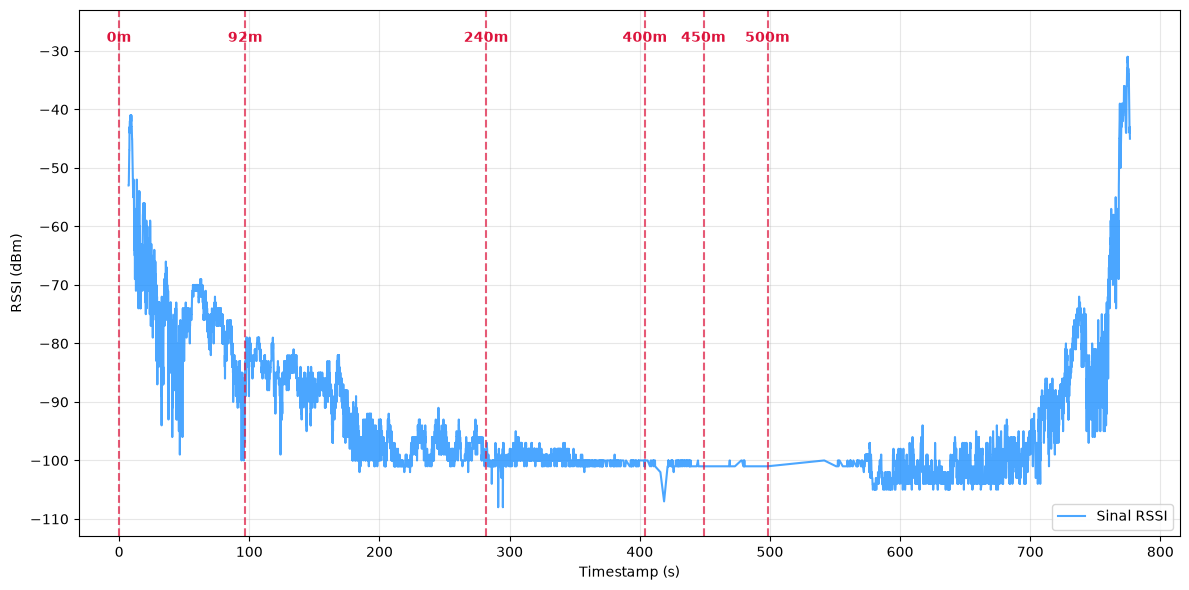
\includegraphics[width=1\textwidth]{images/grafico_rssi.png}\\
    \footnotesize Fonte: Autoria própria, 2026.
\end{figure}

A análise dos arquivos de \textit{log} da estação de solo revelou que, mesmo sob as condições adversas de bloqueio de visada e distanciamento de meio quilômetro, o índice de pacotes invalidados ou corrompidos limitou-se a apenas 1\% do volume total transmitido. Esta margem de erro restrita atesta a alta resiliência da modulação de Espalhamento Espectral por Chirp (CSS - \textit{Chirp Spread Spectrum}) inerente ao protocolo LoRa, que consegue recuperar a carga útil mesmo quando o sinal se encontra próximo ou abaixo do piso de ruído (\textit{noise floor}).

Os pacotes que efetivamente falharam na verificação de redundância cíclica (CRC) devido à corrupção de \textit{bits} foram adequadamente interceptados e descartados pelas rotinas de tratamento de exceção da camada \textit{middleware}, sem ocasionar travamentos no monitoramento geral. Conclui-se, portanto, que a arquitetura de comunicação satisfaz os requisitos do projeto, provendo um alcance operacional robusto que cobre com ampla margem de segurança os raios de giro e as distâncias típicas executadas em competições de aerodesign, onde o voo ocorre majoritariamente em campo aberto e com visada direta desobstruída.
